\section{Indeksy, typy indeksów, statystyki, wykorzystanie przez
         optymalizatory kwerend}
\label{sec:indeksy}

\horrule{0.5pt}
Proszę \underline{omówić budowę} indeksu typu \textbf{drzewo B+}. Proszę
podać wersje tego indeksu (w systemie Microsoft SQL Server: clustered i
non-clustered, w Oracle IOT).\\
\horrule{0.5pt}\\

\textbf{WĘZEŁ WEWNĘTRZNY} z $q-1$ wartości\\

\begin{adjustbox}{width=\columnwidth,center}
    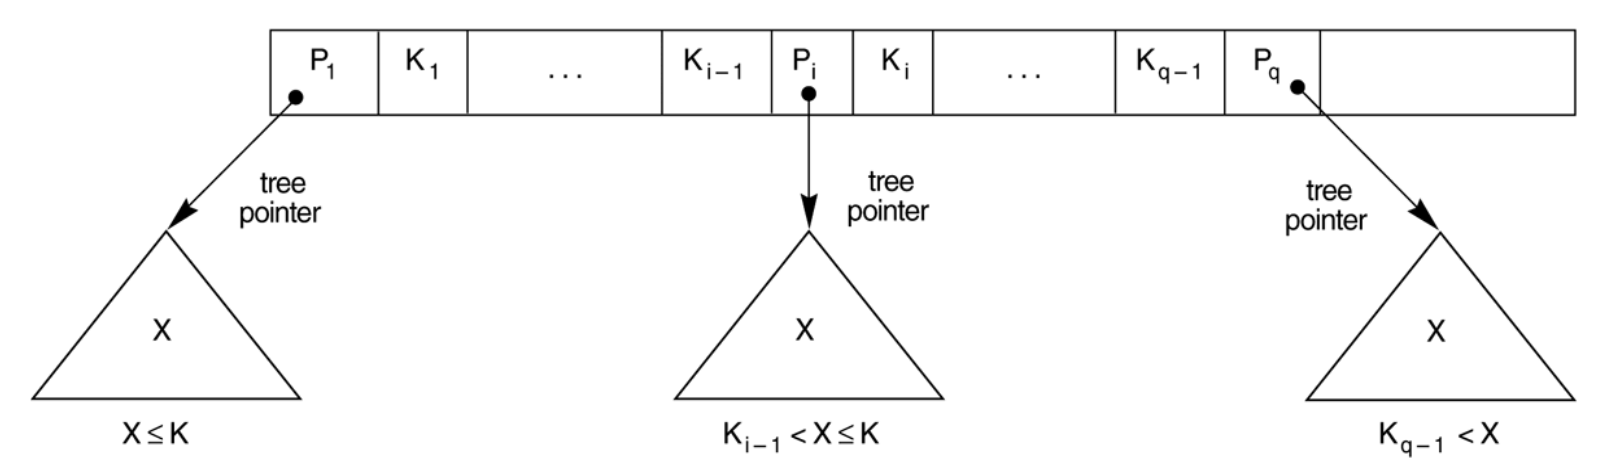
\includegraphics[scale=1]{internal}
\end{adjustbox}

\begin{itemize}
    \item $ \langle P_1, K_1, P_2, K_2, \ldots, P_{q-1}, K_{q-1}, P_q \rangle$,
          gdzie $q \leqslant p$,\\ $P_i (i = 1, \ldots, q)$ jest wskaźnikiem do
          poddrzewa.
    \item $K_1 < K_2 < \ldots < K_{q-1}$
    \item Każdy wewnętrzny węzeł ma co najwyżej $p$ wskaźników.
    \item Każdy węzeł \textit{(z wyjątkiem korzenia)} ma przynajmniej
          $\left\lceil \frac{p}{2} \right\rceil$ wskaźników do poddrzew.\\
          Korzeń ma co najmniej dwa wskaźniki, jeśli jest węzłem
          wewnętrznym.
    \item Węzęł wewnętrzny z $q$ wskaźnikami ma $q-1$ wartości.
\end{itemize}

\pagebreak
\textbf{WĘZEŁ ZEWNĘTRZNY}\\

\begin{adjustbox}{width=\columnwidth,center}
    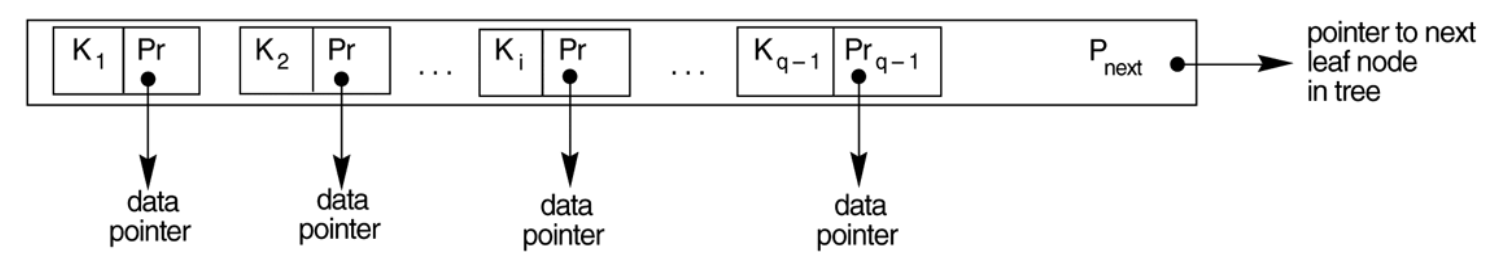
\includegraphics[scale=1]{external}
\end{adjustbox}

\begin{itemize}
    \item $\langle\langle K_1, Pr_1 \rangle , \langle K_2, Pr_2 \rangle ,
     \ldots, \langle K_{q-1}, Pr_{q-1}, \rangle P_{next} \rangle$
          , gdzie $q \leqslant p$ i $Pr_i$ jest wskaźnikiem \textbf{do danych},
          $P_{next}$ wskazuje na następny liść.
    \item $K_1 < K_2 < \ldots < K_{q-1}$
    \item Każdy $Pr_i$ jest wskaźnikiem do danych, który wsakzuje na rekord,
          którego wartość w polu indeksowanym jest równa $K_i$ lub wskazuje
          na blok zawierający rekord lub na blok wskaźników do rekordów z
          takimi samymi wartościami $K_i$ jeśli klucz indeksu nie jest
          unikalny.
    \item Każdy liść przechowuje co najmniej
          $\left\lceil \frac{p}{2} \right\rceil$ wartości.
    \item Wszystkie liście są na tym samym poziomie.

\end{itemize}

% TODO:
% \textbf{WERSJE}\\
% \textbf{B DRZEWO A B+ DRZEWO}\\
